%Version 3.1 December 2024
% See section 11 of the User Manual for version history
%
%%%%%%%%%%%%%%%%%%%%%%%%%%%%%%%%%%%%%%%%%%%%%%%%%%%%%%%%%%%%%%%%%%%%%%
%%                                                                 %%
%% Please do not use \input{...} to include other tex files.       %%
%% Submit your LaTeX manuscript as one .tex document.              %%
%%                                                                 %%
%% All additional figures and files should be attached             %%
%% separately and not embedded in the \TeX\ document itself.       %%
%%                                                                 %%
%%%%%%%%%%%%%%%%%%%%%%%%%%%%%%%%%%%%%%%%%%%%%%%%%%%%%%%%%%%%%%%%%%%%%

%%\documentclass[referee,sn-basic]{sn-jnl}% referee option is meant for double line spacing

%%=======================================================%%
%% to print line numbers in the margin use lineno option %%
%%=======================================================%%

%%\documentclass[lineno,pdflatex,sn-basic]{sn-jnl}% Basic Springer Nature Reference Style/Chemistry Reference Style

%%=========================================================================================%%
%% the documentclass is set to pdflatex as default. You can delete it if not appropriate.  %%
%%=========================================================================================%%

%%\documentclass[sn-basic]{sn-jnl}% Basic Springer Nature Reference Style/Chemistry Reference Style

%%Note: the following reference styles support Namedate and Numbered referencing. By default the style follows the most common style. To switch between the options you can add or remove Numbered in the optional parenthesis. 
%%The option is available for: sn-basic.bst, sn-chicago.bst%  
 
%%\documentclass[pdflatex,sn-nature]{sn-jnl}% Style for submissions to Nature Portfolio journals
%%\documentclass[pdflatex,sn-basic]{sn-jnl}% Basic Springer Nature Reference Style/Chemistry Reference Style
\documentclass[pdflatex,sn-mathphys-num]{sn-jnl}% Math and Physical Sciences Numbered Reference Style
%%\documentclass[pdflatex,sn-mathphys-ay]{sn-jnl}% Math and Physical Sciences Author Year Reference Style
%%\documentclass[pdflatex,sn-aps]{sn-jnl}% American Physical Society (APS) Reference Style
%%\documentclass[pdflatex,sn-vancouver-num]{sn-jnl}% Vancouver Numbered Reference Style
%%\documentclass[pdflatex,sn-vancouver-ay]{sn-jnl}% Vancouver Author Year Reference Style
%%\documentclass[pdflatex,sn-apa]{sn-jnl}% APA Reference Style
%%\documentclass[pdflatex,sn-chicago]{sn-jnl}% Chicago-based Humanities Reference Style

%%%% Standard Packages
%%<additional latex packages if required can be included here>

\usepackage{graphicx}%
\usepackage{multirow}%
\usepackage{amsmath,amssymb,amsfonts}%
\usepackage{amsthm}%
\usepackage{mathrsfs}%
\usepackage[title]{appendix}%
\usepackage{xcolor}%
\usepackage{textcomp}%
\usepackage{manyfoot}%
\usepackage{booktabs}%
\usepackage{algorithm}%
\usepackage{algorithmicx}%
\usepackage{algpseudocode}%
\usepackage{listings}%
\usepackage{subcaption}

\lstset{
    basicstyle=\footnotesize\ttfamily,
    breaklines=true,
    breakatwhitespace=true,
    columns=fullflexible,
    frame=single,
    showstringspaces=false
}
%%%%

%%%%%=============================================================================%%%%
%%%%  Remarks: This template is provided to aid authors with the preparation
%%%%  of original research articles intended for submission to journals published 
%%%%  by Springer Nature. The guidance has been prepared in partnership with 
%%%%  production teams to conform to Springer Nature technical requirements. 
%%%%  Editorial and presentation requirements differ among journal portfolios and 
%%%%  research disciplines. You may find sections in this template are irrelevant 
%%%%  to your work and are empowered to omit any such section if allowed by the 
%%%%  journal you intend to submit to. The submission guidelines and policies 
%%%%  of the journal take precedence. A detailed User Manual is available in the 
%%%%  template package for technical guidance.
%%%%%=============================================================================%%%%

%% as per the requirement new theorem styles can be included as shown below
\theoremstyle{thmstyleone}%
\newtheorem{theorem}{Theorem}%  meant for continuous numbers
%%\newtheorem{theorem}{Theorem}[section]% meant for sectionwise numbers
%% optional argument [theorem] produces theorem numbering sequence instead of independent numbers for Proposition
\newtheorem{proposition}[theorem]{Proposition}% 
%%\newtheorem{proposition}{Proposition}% to get separate numbers for theorem and proposition etc.

\theoremstyle{thmstyletwo}%
\newtheorem{example}{Example}%
\newtheorem{remark}{Remark}%

\theoremstyle{thmstylethree}%
\newtheorem{definition}{Definition}%

\raggedbottom
%%\unnumbered% uncomment this for unnumbered level heads

\begin{document}

\title[QR-Wanbot Development]{QR-Wanbot: Balancing Agility and Energy Efficiency in a Servo-Driven 12-DOF Quadruped Robot}

%%=============================================================%%
%% GivenName	-> \fnm{Joergen W.}
%% Particle	-> \spfx{van der} -> surname prefix
%% FamilyName	-> \sur{Ploeg}
%% Suffix	-> \sfx{IV}
%% \author*[1,2]{\fnm{Joergen W.} \spfx{van der} \sur{Ploeg} 
%%  \sfx{IV}}\email{iauthor@gmail.com}
%%=============================================================%%

\author[1]{\fnm{Anas} \sur{Aburaya}}

\author*[1]{\fnm{Mohd Ridzuan} \sur{Ahmed}}\email{mdridzuan@utm.my}

\affil*[1]{\orgdiv{Department of Control and Mechatronics, Faculty of Electrical Engineering}, \orgname{Universiti Teknologi Malaysia}, \orgaddress{\city{Skudai}, \postcode{81300}, \state{Johor}, \country{Malaysia}}}


%%==================================%%
%% Sample for unstructured abstract %%
%%==================================%%

\abstract{This paper presents the development and control of QR-Wanbot, a cost-effective 12-DOF quadruped robot designed for agile dynamic locomotion. We address the challenge of achieving high-performance actuation on a constrained budget by validating a novel high-voltage (8.4V) servo-based drive system. The mechanical design features a custom belt-reduced transmission that isolates leg inertia, enabling rapid swing phases essential for dynamic gaits. The control architecture is built on a real-time STM32F4 embedded system running FreeRTOS, effectively separating high-level gait planning from high-frequency kinematic stabilization. A robust Trot gait is generated using a distinct two-phase diagonal trajectory planner coupled with active IMU-based attitude correction. We provide a comprehensive derivation of the inverse kinematics and trajectory generation logic. Finally, we propose a rigorous experimental framework to quantify the robot's omnidirectional agility and energy efficiency, positioning the QR-Wanbot as an accessible yet capable platform for legged robotics research.}

%%================================%%
%% Sample for structured abstract %%
%%================================%%

% \abstract{\textbf{Purpose:} The abstract serves both as a general introduction to the topic and as a brief, non-technical summary of the main results and their implications. The abstract must not include subheadings (unless expressly permitted in the journal's Instructions to Authors), equations or citations. As a guide the abstract should not exceed 200 words. Most journals do not set a hard limit however authors are advised to check the author instructions for the journal they are submitting to.
% 
% \textbf{Methods:} The abstract serves both as a general introduction to the topic and as a brief, non-technical summary of the main results and their implications. The abstract must not include subheadings (unless expressly permitted in the journal's Instructions to Authors), equations or citations. As a guide the abstract should not exceed 200 words. Most journals do not set a hard limit however authors are advised to check the author instructions for the journal they are submitting to.
% 
% \textbf{Results:} The abstract serves both as a general introduction to the topic and as a brief, non-technical summary of the main results and their implications. The abstract must not include subheadings (unless expressly permitted in the journal's Instructions to Authors), equations or citations. As a guide the abstract should not exceed 200 words. Most journals do not set a hard limit however authors are advised to check the author instructions for the journal they are submitting to.
% 
% \textbf{Conclusion:} The abstract serves both as a general introduction to the topic and as a brief, non-technical summary of the main results and their implications. The abstract must not include subheadings (unless expressly permitted in the journal's Instructions to Authors), equations or citations. As a guide the abstract should not exceed 200 words. Most journals do not set a hard limit however authors are advised to check the author instructions for the journal they are submitting to.}

\keywords{Quadruped Robot, STM32, FreeRTOS, Inverse Kinematics, Legged Locomotion}

%%\pacs[JEL Classification]{D8, H51}

%%\pacs[MSC Classification]{35A01, 65L10, 65L12, 65L20, 65L70}

\maketitle

\section{Introduction}\label{sec1}

The field of mobile robotics has seen a paradigm shift in recent years, moving from simple wheeled platforms to complex legged systems capable of traversing unstructured environments. Legged robots, and particularly quadrupeds, draw inspiration from biological counterparts to offer superior terrain maneuverability. Unlike wheels or tracks, legs can step over obstacles, climb stairs, and adjust their height to navigate low-clearance passages. This versatility makes them ideal candidates for applications in search and rescue (SAR) missions, hazardous environment inspection, and last-mile logistics \cite{Fan2024}.

However, the development of small-scale, agile, and power-efficient quadruped robots presents a significant engineering challenge. It requires a holistic optimization of mechanical design, actuator selection, and control software. A primary constraint in this domain is the trade-off between dynamic performance (agility) and energy efficiency (operating time). Traditional hydraulic actuators, used in pioneering robots like BigDog \cite{Raibert2008}, offer immense power density but suffer from high weight, acoustic noise, and hydraulic leakage issues, rendering them unsuitable for compact platforms.

Electric actuation has thus become the standard for small-to-medium-sized quadrupeds. This category is currently dominated by two distinct design philosophies: Quasi-Direct Drive (QDD) brushless motors and standard geared servo motors. High-performance platforms such as the MIT Cheetah series \cite{Bosworth2015} and the Stanford Doggo \cite{Kau2019} utilize high-torque brushless motors coupled with low-ratio planetary gearboxes (QDD). This configuration provides high bandwidth, transparency (back-drivability), and proprioceptive capabilities, enabling dynamic gaits like trotting and backflipping. However, QDD systems typically have low torque constants ($K_t$), requiring high continuous currents to maintain posture, which severely impacts battery life. Furthermore, they require specialized driver hardware (e.g., ODrive) and complex calibration, inflating the system cost.

On the other end of the spectrum, hobbyist and educational robots often employ commercial off-the-shelf (COTS) RC servo motors. These units integrate a DC motor, gear train, and position controller into a compact package. While cost-effective and easy to interface with, standard 5V/6V servos generally lack the torque-to-weight ratio and speed required for stable dynamic locomotion, often relegating such robots to slow, static walking gaits.

This paper presents the design, development, and control of the QR-Wanbot, a 12-degree-of-freedom (DOF) quadruped robot that aims to bridge the gap between low-cost hobbyist platforms and high-end research robots. By utilizing modern high-voltage (8.4V) serial bus servos and a custom optimized leg mechanism, we achieve a balance of agility and endurance not found in comparable systems. We detail the transition from a single-leg experimental validation phase to the construction of the full robot, and we present a comprehensive embedded control architecture based on the STM32F4 microprocessor and FreeRTOS.

\section{Related Work}\label{sec:related}

The development of the QR-Wanbot builds upon a rich history of legged robotics research, which has been extensively summarized in recent surveys \cite{Fan2024, Chai2022}. These reviews categorize the field into three primary actuation domains: hydraulic, brushless electric, and servo-based.

\subsection{Hydraulic Quadrupeds}
Early successful dynamic quadrupeds utilized hydraulic actuation due to its high power density. BigDog \cite{Raibert2008}, developed by Boston Dynamics, demonstrated unprecedented rough-terrain capability but was heavy (109 kg) and powered by an internal combustion engine. The HyQ series \cite{Semini2011, Semini2017} and HyQ2Max \cite{Semini2015} further refined hydraulic locomotion, demonstrating robust dynamic gaits. Efforts to miniaturize this technology resulted in the MiniHyQ \cite{Khan2015}, which lowered the weight to 35kg but still suffered from the complexity of hydraulic lines and pumps. Recent research into electro-hydrostatic actuators \cite{Nakanishi2021} attempts to bridge this gap, but hydraulic solutions remain largely impractical for small-scale (<10kg) robots.

\subsection{Brushless Electric Quadrupeds}
The shift to electric actuation was led by the MIT Cheetah series, starting with foundational work on high-speed bounding in Cheetah 2 \cite{Park2017} and robust control in Cheetah 3 \cite{Bledt2018}. This culminated in the MIT Mini Cheetah \cite{Katz2019} and the Super Mini Cheetah \cite{Bosworth2015}, which utilized proprioceptive actuators to enable backflips and high-speed running. The commercial sector has seen success with platforms like ANYmal \cite{Hutter2016} and Boston Dynamics' Spot \cite{Bouman2020}, as well as the Unitree Go2 \cite{UnitreeGo2}, which perform complex tasks but at a high cost. In the open-source domain, the Stanford Doggo \cite{Kau2019} popularized the coaxial mechanism for jumping, though its power consumption (0.698 W/g) remains high.

\subsection{Servo-Based and Low-Cost Designs}
To address the cost and efficiency barriers, researchers have explored servo-based designs. The Monash Dingo \cite{Alex2023} and PuppyPi \cite{PuppyPi2024} successfully utilize hobby servos for locomotion but are often torque-limited. Recent open-source initiatives such as the Q8bot 2 \cite{Q8bot2025} and Mjukost \cite{Mjukost2023} have further democratized quadruped research by utilizing modular, accessible components. Similarly, educational platforms like Q-Robot \cite{QRobot2025} demonstrate the viability of 12-DOF systems for teaching kinematics. Modular service robots \cite{ServiceQuad2025} have also begun to adopt servo actuation for lightweight tasks. Several studies have focused on optimizing single-leg structures \cite{Chen2020, Chen2021} and analyzing the structural design of small quadrupeds \cite{Shi2021, Fredriksson2021}. Rahman et al. \cite{Rahman2023} provided a computational simulation for a 12-DOF servo quadruped, laying the groundwork for low-cost development. Other specialized designs include the cat-like Aquro \cite{Saputra2021} and robots utilizing topology-optimized compliant legs \cite{Sun2023} to improve efficiency. Our work integrates the dynamic modeling principles formulated by Khalil \cite{Khalil2011} to maximize the performance of these servo-driven systems.

\section{Mechanical Design and Analysis}\label{sec2}

The QR-Wanbot features a modular design with a central chassis and four identical 3-DOF legs. The system integration is depicted in Figure \ref{fig:hardware}, which illustrates the high-level hardware architecture. The central STM32F411RE microcontroller acts as the brain, interfacing directly with the sensors and actuator drivers. Power is supplied by a 2S 8.4V LiPo battery, which drives the high-voltage servos directly to maximize torque and efficiency, while a regulated 5V rail powers the logic circuits.

\begin{figure}[h]
\centering
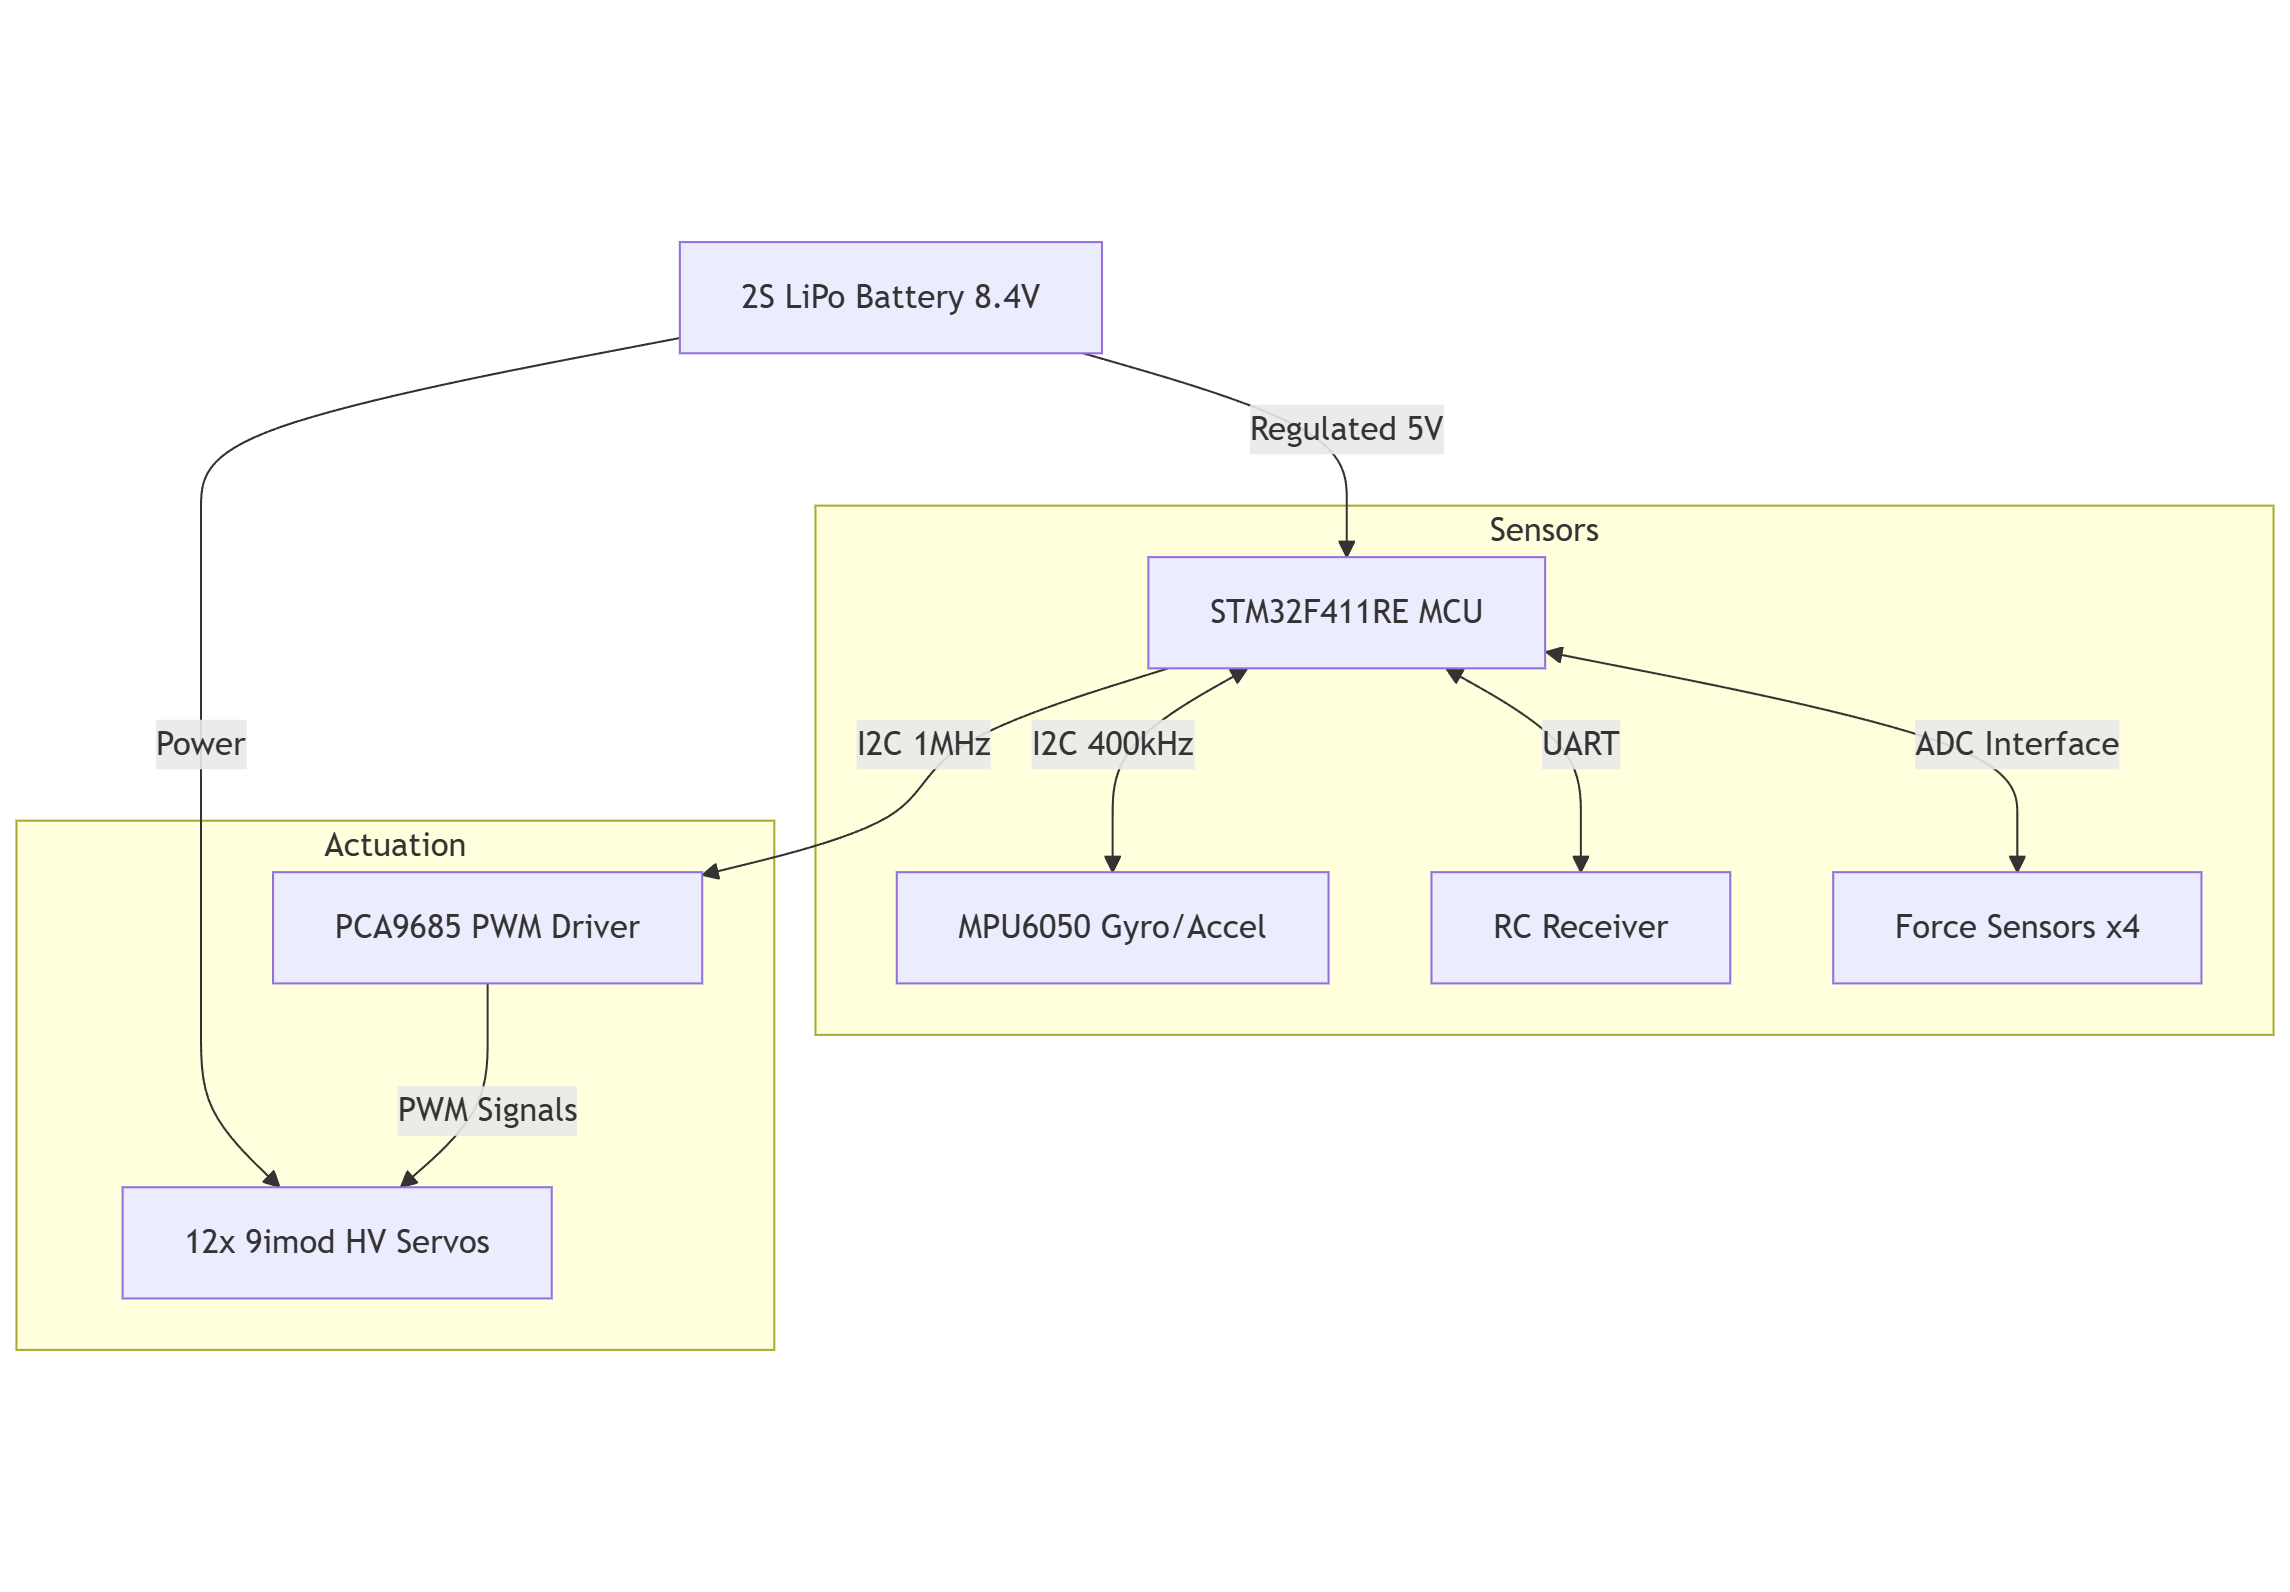
\includegraphics[width=0.9\textwidth]{hardware.png}
\caption{System Hardware Architecture: The STM32F411 central controller interfaces with the MPU6050 IMU for state estimation and the PCA9685 driver for actuator control. High-voltage servos are powered directly from the LiPo source, and FSRs monitor ground contact.}
\label{fig:hardware}
\end{figure}

The mechanical layout of the robot is designed for compactness and serviceability. Figure \ref{fig:iso_view} shows the isometric view of the complete assembly.

\begin{figure}[h]
\centering
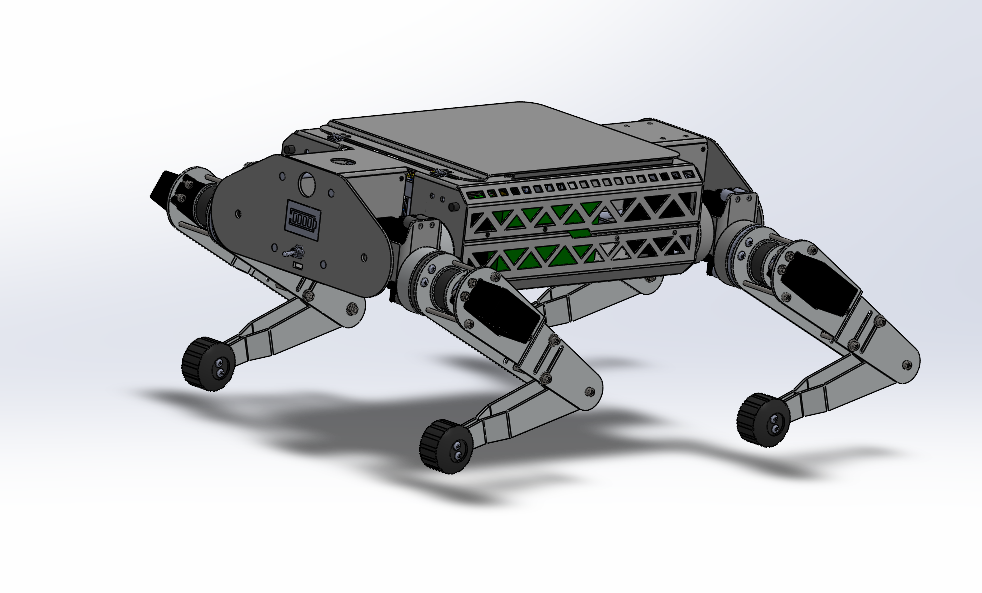
\includegraphics[width=0.8\textwidth]{robot_3D_design_isometric.png}
\caption{Isometric view of the QR-Wanbot CAD model, showing the component layout.}
\label{fig:iso_view}
\end{figure}

The core of the mechanical design is the choice of the 9imod high-voltage digital servo. These motors were selected specifically for their ability to operate directly from a 2S LiPo battery at 8.4V, which results in a lower current draw for the same power output compared to standard 6V servos. Each servo provides a substantial stall torque of 5.8 Nm (approx. 60 kg-cm) and a speed of 0.12 seconds per 60 degrees. Communication is handled via a standard PWM interface, compatible with the PCA9685 drivers used in the system.

Each leg consists of a Hip Roll (abduction/adduction) joint, a Hip Pitch joint, and a Knee Pitch joint. A critical design decision was to minimize the rotational inertia of the leg, which is essential for achieving the rapid swing phases required for trotting. To achieve this, the heavy knee motor was not placed at the knee joint itself but was co-located with the hip pitch motor at the "shoulder" of the leg. Torque is transferred to the knee joint via a timing belt transmission with a 1.25:1 reduction ratio. This reduction slightly amplifies the motor torque from 5.8 Nm to 7.25 Nm at the knee, providing a margin for vertical impulse generation. The upper leg link features slotted motor mounts, allowing the motor position to be fine-tuned to tension the belt effectively, preventing tooth skipping under load.

 Structurally, the robot utilizes a hybrid material approach. The main leg links and chassis plates are fabricated from aluminum alloy, offering the necessary rigidity to prevent link flexing under load, which would otherwise complicate the kinematic control. The foot tips, however, are made of silicone. These act as passive compliant elements or damped springs, absorbing high-frequency impact shocks during foot-stride and increasing friction with the ground to prevent slippage.

To further illustrate the mechanical configuration, Figure \ref{fig:ortho_views} presents the orthographic projections of the robot.

\begin{figure}[h]
\centering
\begin{subfigure}[b]{0.3\textwidth}
    \centering
    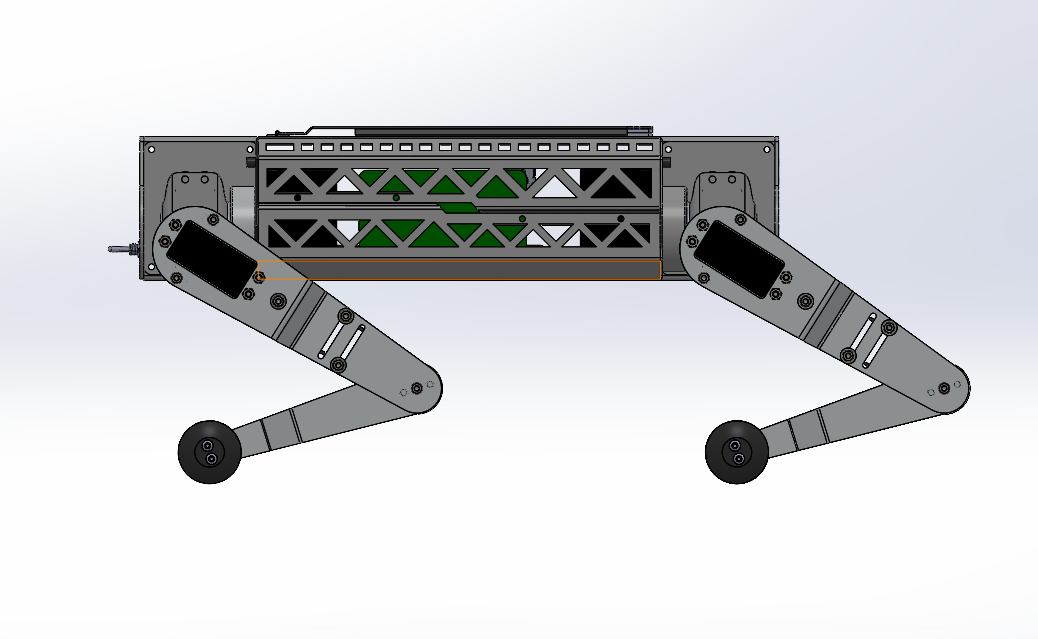
\includegraphics[width=\textwidth]{robot_side.png}
    \caption{Side View}
    \label{fig:side_view}
\end{subfigure}
\hfill
\begin{subfigure}[b]{0.3\textwidth}
    \centering
    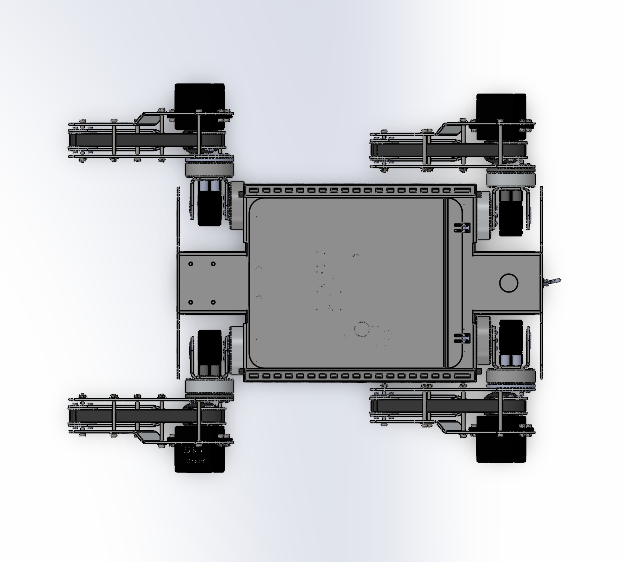
\includegraphics[width=\textwidth]{robot_top.png}
    \caption{Top View}
    \label{fig:top_view}
\end{subfigure}
\hfill
\begin{subfigure}[b]{0.3\textwidth}
    \centering
    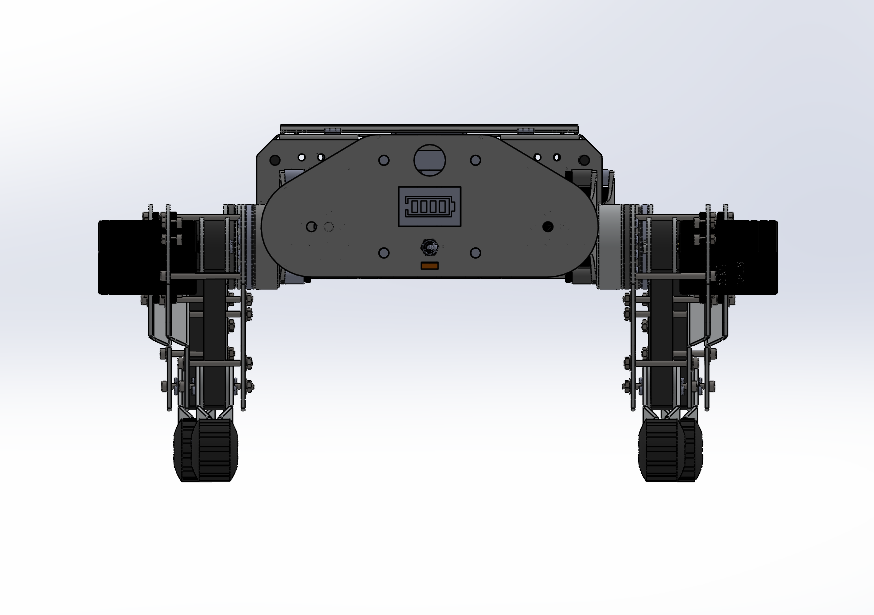
\includegraphics[width=\textwidth]{robot_back.png}
    \caption{Back View}
    \label{fig:back_view}
\end{subfigure}
\caption{Design views of the QR-Wanbot: (a) Side View, (b) Top View, and (c) Back View.}
\label{fig:ortho_views}
\end{figure}

\section{Control System Architecture}\label{sec3}

The control framework is designed to be modular, deterministic, and computationally efficient, running on an STM32F411RE microcontroller. Robotic control involves managing tasks with varying timing requirements, and we utilize FreeRTOS to schedule these tasks preemptively. The software architecture, shown in Figure \ref{fig:software}, creates a clear separation of concerns between high-level logic and real-time control.

\begin{figure}[h]
\centering
\includegraphics[width=1.0\textwidth]{{Software Control Architecture}.png}
\caption{Software Control Architecture: Data flow between the low-frequency MainTask (Gait Logic) and the high-frequency CalcTask (Real-time Control). Sensor fusion and Inverse Kinematics occur within the strict 50Hz scheduling loop to ensure stable motion.}
\label{fig:software}
\end{figure}

The software is structured around two primary tasks. The first is the \texttt{MainTask}, which operates at a normal priority and a frequency of roughly 10 Hz. This task is responsible for high-level decision-making and state machine management, as detailed in Figure \ref{fig:fsm}. It interprets incoming UART packets from the remote controller, maps joystick values ($J_x, J_y$) to velocity vectors ($\dot{x}, \dot{y}, \dot{\theta}_z$), and manages the specific transitions within the Trot gait cycle. Note that the FSM includes specific initialization and safety states (SafeStop) to handle low-battery or fall scenarios.

\begin{figure}[h]
\centering
\includegraphics[width=1.0\textwidth]{{Finite State Machine}.png}
\caption{Trot Gait Finite State Machine (FSM): A detailed view of the Trot lifecycle. The system initializes, calibrates sensors, and enters a Standby state. Upon joystick input, it enters the Trot loop, alternating between diagonal pair swing phases (Phase A and Phase B) to generate forward motion.}
\label{fig:fsm}
\end{figure}
These readings to obtain the robot's absolute roll ($\phi$) and pitch ($\theta$) orientation. Following this, the gait generator updates the foot tip trajectories based on the current phase of the gait cycle. The active stabilization block then computes PID outputs to adjust leg lengths to maintain balance. Finally, the Inverse Kinematics engine solves for the required joint angles, and the actuation layer updates the PWM duty cycles via the PCA9685 driver.

\subsection{Mathematical Formulation}

\subsubsection{Inverse Kinematics (IK) Derivation}

The Inverse Kinematics (IK) solver is the fundamental component of the locomotion engine. Its purpose is to transform a desired foot tip position in Cartesian coordinates $P_{target} = [x, y, z]^T$ (relative to the robot's center of mass or hip attachment point) into the necessary joint angles for the three motors: $\theta_1$ (Hip Roll), $\theta_2$ (Hip Pitch), and $\theta_3$ (Knee Pitch).

The mechanical structure of the QR-Wanbot leg is a standard 3-DOF configuration with a lateral offset at the hip. To solve the kinematics, we strictly decouple the lateral motion (Roll) from the sagittal motion (Pitch) using a projection method. The derivation is performed in three methodical steps:

First, the global body-frame coordinates are transformed into the local leg frame. Let the center of the robot be the origin $(0,0,0)$. For a given leg $i$, its hip attachment point is located at $(L/2, W/2)$ for the FL leg. The target vector $P_{leg}$ relative to the shoulder pivot is:
\begin{equation}
    P_{leg} = P_{global} - P_{shoulder}
\end{equation}
Furthermore, to stabilize the robot body under rotation, we apply a counter-rotation transform. If the body has a Roll $\phi$ and Pitch $\theta$, the effective target point must be adjusted to keep the foot planted:
\begin{equation}
    \begin{bmatrix} x' \\ y' \\ z' \end{bmatrix} = R_y(\theta)^T R_x(\phi)^T \begin{bmatrix} x \\ y \\ z \end{bmatrix}
\end{equation}
This ensures that when the body tilts, the feet move purely vertically relative to the ground plane to maintain contact.

The Hip Roll joint ($\theta_1$) is responsible for the lateral position $y$ of the foot. The leg structure includes a fixed mechanical offset $d_{offset}$ (the distance from the roll axis to the pitch axis). This creates a geometric constraint in the $YZ$ plane. The distance from the roll pivot to the foot tip is defined as the hypotenuse $H_{yz}$:
\begin{equation}
    H_{yz} = \sqrt{y'^2 + z'^2}
\end{equation}
Notice that the leg cannot reach the origin of the rolling plane due to the offset $d_{offset}$. The foot tip typically resides on a tangent to the circle of radius $d_{offset}$. We construct a triangle with hypotenuse $H_{yz}$ and one side equal to $d_{offset}$. The remaining side, which represents the effective length of the leg projected onto the pitch plane, is:
\begin{equation}
    L_{proj} = \sqrt{H_{yz}^2 - d_{offset}^2}
\end{equation}
The magnitude of the Roll angle is the superposition of the geometric angle to the point and the offset angle required to span $d_{offset}$.
\begin{equation}
    \alpha_{geom} = \arctan2(y', z')
\end{equation}
\begin{equation}
    \alpha_{offset} = \arctan2(L_{proj}, d_{offset})
\end{equation}
Thus, the final Hip Roll angle is:
\begin{equation}
    \theta_1 = \alpha_{geom} + \alpha_{offset}
\end{equation}
(Note: Depending on the leg index (left vs. right), the sign of the offset term may be inverted).

Once $\theta_1$ is determined, the problem reduces to a 2-D planar arm with link lengths $l_1$ (Upper Leg) and $l_2$ (Lower Leg). The target point in this plane is defined by the forward coordinate $x'$ and the projected vertical length $L_{proj}$ derived in Step 2.
The Euclidean distance from the hip pitch axis to the foot tip is:
\begin{equation}
    H_{sac} = \sqrt{x'^2 + L_{proj}^2}
\end{equation}
This distance $H_{sac}$ forms a triangle with the two limb segments $l_1$ and $l_2$. We apply the Law of Cosines to solve for the interior knee angle $\gamma_{knee}$:
\begin{equation}
    H_{sac}^2 = l_1^2 + l_2^2 - 2 l_1 l_2 \cos(\pi - \theta_3)
\end{equation}
Rearranging for $\theta_3$ (Interior Knee Angle):
\begin{equation}
    \theta_3 = \pi - \arccos\left( \frac{l_1^2 + l_2^2 - H_{sac}^2}{2 l_1 l_2} \right)
\end{equation}
For the Hip Pitch angle $\theta_2$, we sum the angle to the target vector and the interior angle of the first link:
\begin{equation}
    \beta_{target} = \arctan2(x', L_{proj})
\end{equation}
\begin{equation}
    \beta_{interior} = \arccos\left( \frac{l_1^2 + H_{sac}^2 - l_2^2}{2 l_1 H_{sac}} \right)
\end{equation}
Resulting in:
\begin{equation}
    \theta_2 = \beta_{target} + \beta_{interior}
\end{equation}
These three angles $(\theta_1, \theta_2, \theta_3)$ are computed at 50Hz for all four legs, accounting for individual leg offsets and motion limits.


\subsubsection{Gait Trajectory Generation}
To ensure smooth locomotion, we implement defined trajectories for the foot tips. For the planar ($xy$) movement, we utilize a linear interpolation between the start and end points of the stride:
\begin{equation}
    P_{xy}(t) = P_{start} + (P_{end} - P_{start}) \times t_{phase}
\end{equation}
For the vertical ($z$) foot clearance during the swing phase, we employ a parabolic profile (equivalent to a Bezier curve) to minimize impact forces. The height $Z(t)$ is given by:
\begin{equation}
    Z(t) = 4 H_{step} \cdot t_{swing} \cdot (1 - t_{swing})
\end{equation}
Where $H_{step}$ is the maximum step height and $t_{swing} \in [0, 1]$ is the normalized time of the swing phase.

\subsubsection{Signal Smoothing}
To prevent jitter from the inverse kinematics solutions, we apply an Exponential Moving Average (EMA) filter to the target foot positions before actuation:
\begin{equation}
```
    P_{smoothed}[k] = \alpha \cdot P_{target}[k] + (1 - \alpha) \cdot P_{smoothed}[k-1]
\end{equation}
Where $\alpha$ is the smoothing factor (experimentally tuned to 0.7 for optimal responsiveness vs. smoothness).


\section{Experimental Results}\label{sec4}

To fully evaluate the capabilities of the completed 12-DOF QR-Wanbot, we conducted a series of experiments designed to quantify its agility, stability, and energy efficiency.

\subsection{Locomotion Analysis}
The robot's velocity was evaluated at three distinct gait cycle durations: 683 ms, 820 ms, and 1025 ms. The experimental setup for these tests is shown in Figure \ref{fig:locomotion_test}. Through these tests, we recorded a minimum speed of 0.028 m/s and a maximum achievable speed of 0.088 m/s. Furthermore, we analyzed the robot's ability to maintain a straight trajectory during locomotion. The deviation from the ideal path is visually represented in Figure \ref{fig:deviation}, demonstrating the performance of the open-loop gait integrator.

\begin{figure}[h]
\centering
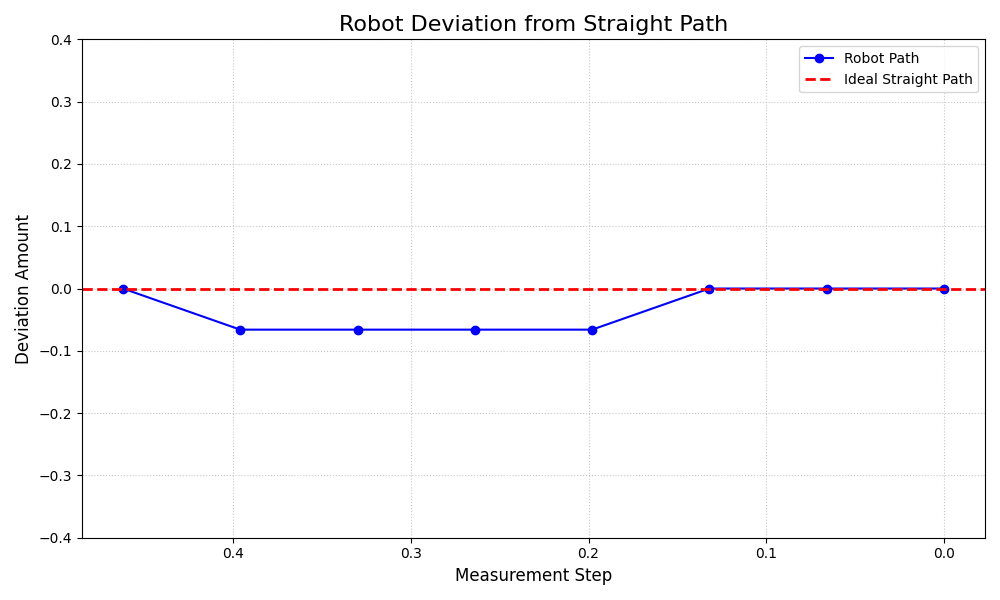
\includegraphics[width=0.65\textwidth]{deviation_graph.png}
\caption{Robot deviation from a straight path during locomotion.}
\label{fig:deviation}
\end{figure}

\begin{figure}[h]
\centering
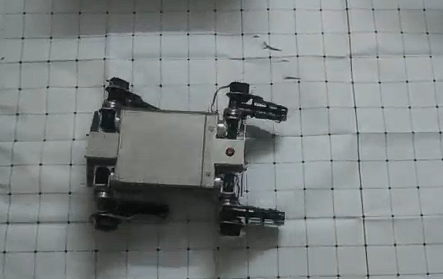
\includegraphics[width=0.65\textwidth]{locomotion_test.png}
\caption{Experimental setup for the locomotion analysis tests.}
\label{fig:locomotion_test}
\end{figure}

\subsection{Stability Analysis}
To validate the efficacy of the control system, we tested the IMU-based active stabilization loop. Figure \ref{fig:imu_graph} illustrates the pitch and roll stability of the robot during operation, highlighting the system's ability to maintain a level torso. The experimental setup used to apply disturbances and measure stability is depicted in Figure \ref{fig:stability_analysis}.

\begin{figure}[h]
\centering
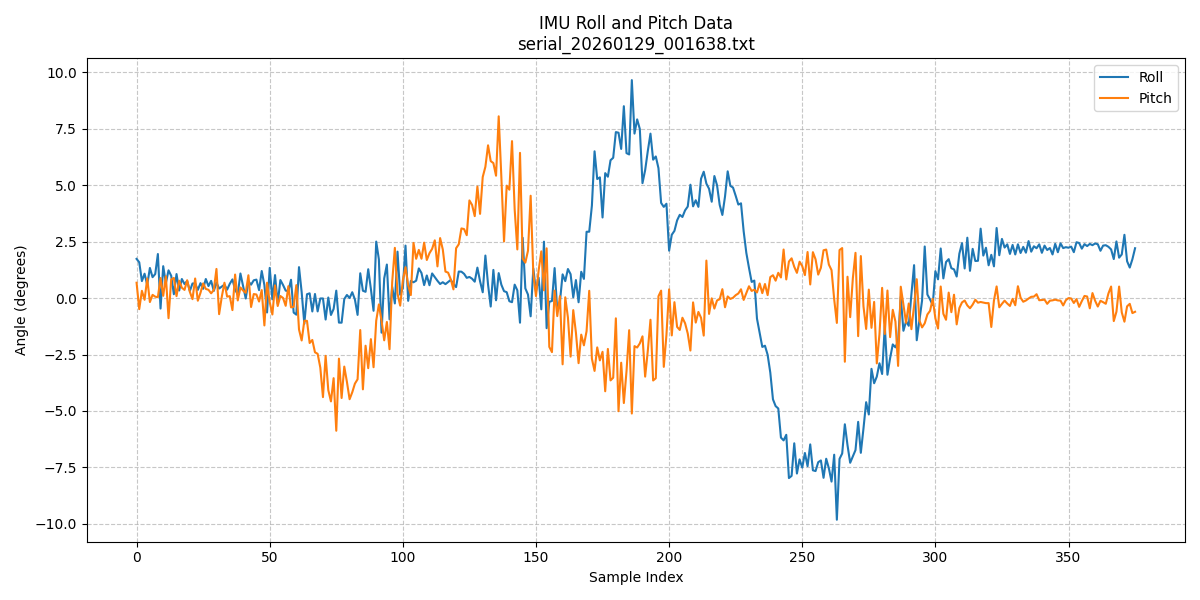
\includegraphics[width=0.75\textwidth]{IMU_Pitch_Roll.png}
\caption{IMU Pitch and Roll response, demonstrating active stabilization.}
\label{fig:imu_graph}
\end{figure}

\begin{figure}[h]
\centering
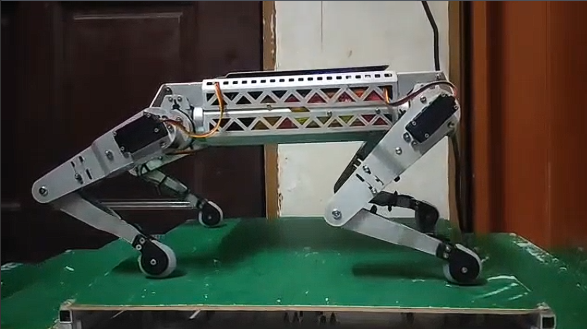
\includegraphics[width=0.75\textwidth]{stability_analysis.png}
\caption{Experimental setup for the stability analysis tests.}
\label{fig:stability_analysis}
\end{figure}

\subsection{Power Consumption and Efficiency}
Energy efficiency is a critical metric for autonomous platforms, and thus we measured the power consumption both at standing positions and during motion. The recorded power usage ranged from a minimum of 19.7 W to a maximum of 135.7 W, with an average power consumption of approximately 80 W. Based on these measurements and a maximum speed of 0.088 m/s, the Cost of Transport (CoT) was calculated as shown in Equation \ref{eq:cot}:
\begin{equation}
    CoT = 80 \times 3 \times 9.81 \times 0.088 = 207.18
    \label{eq:cot}
\end{equation}


\section{Discussion}\label{sec5}
The design analysis suggests that the QR-Wanbot is well-positioned to bridge the gap between hobbyist toys and professional research platforms. The theoretical analysis of the 8.4V servo architecture indicates a significant advantage in holding torque compared to direct-drive brushless systems, potentially offering higher efficiency for static or low-speed maneuvers. The belt reduction mechanism is designed to isolate knee inertia, which we anticipate will enable rapid gait cycles ($\approx$ 100ms) once validated.
However, limitations remain in the current sensor suite. The lack of torque feedback prevents true impedance control. The robot currently relies on kinematic rigidity and the passive compliance of the TPU feet. The proposed experiments will be crucial in determining if this open-loop stability is sufficient for rough terrain traversal.


\section{Conclusion}\label{sec6}
We have presented the Development and Control Control architecture of the QR-Wanbot. By leveraging a high-voltage servo architecture controlled by a real-time FreeRTOS system, we designed a platform optimized for low-cost research. We detailed the mechanical transformation from a single servomotor to a 12-DOF quadruped and provided a comprehensive mathematical formulation for the inverse kinematics and gait generation. The proposed experimental framework outlines a rigorous path to validating the robot's agility, stability, and energy efficiency. This work serves as a blueprint for calculating and constructing high-performance servo-based quadrupeds. Future work will focus on executing the proposed validation plan and integrating force-feedback sensors to enable advanced impedance control strategies.


\backmatter

\bmhead{Acknowledgements}
We acknowledge the support of the Universiti Teknologi Malaysia robotics lab facilities.

\section*{Declarations}
Funding: Not applicable. Conflict of interest: The authors declare no competing interests.

\begin{appendices}

\section{Gait Controller Logic}\label{secA2}
\begin{lstlisting}[language=C]
void leg_cycle(float positions[], uint8_t leg, uint8_t mode, uint32_t ticks, 
               float x_setpoint, float y_setpoint, float angles[], 
               float p, float r, float yaw) {
    float adjusted_time_in_cycle = (double)(ticks % step_pace) / (float)step_pace;
    
    // Phase Shift for Diagonal Pairs (Trot)
    if (mode == TROT && (leg == 2 || leg == 3)) {
        adjusted_time_in_cycle = fmod(adjusted_time_in_cycle + 0.5, 1.0);
    }

    uint8_t time_is_swing = (adjusted_time_in_cycle < TROT_SWING_END);

    if (time_is_swing && !landed_early[leg]) {
        // --- SWING PHASE ---
        float swing_progress = adjusted_time_in_cycle / TROT_SWING_END;
        
        // Active Balance Correction
        float corrective_x = pitch_error * K_PITCH_BALANCE_X; 
        float corrective_y = roll_error * K_ROLL_BALANCE_Y;

        positions[0] = generate_linear_xy_trajectory(-x_setpoint, 
                                     x_setpoint + corrective_x, swing_progress);
        positions[1] = generate_linear_xy_trajectory(-y_setpoint, 
                                     y_setpoint + corrective_y, swing_progress);

        // Generate Parabolic Z Profile
        float base_z = generate_cubic_z_trajectory(swing_progress);
        positions[2] = body_height - base_z;

        // Yaw correction during swing
        angles[2] = generate_linear_xy_trajectory(-yaw, yaw, swing_progress);

    } else {
        // --- STANCE PHASE ---
        float raw_progress = (adjusted_time_in_cycle - TROT_SWING_END) / 
                             (1.0f - TROT_SWING_END);
        float stance_progress = fmaxf(0.0f, raw_progress);

        // Move leg backwards relative to body to generate forward motion
        positions[0] = generate_linear_xy_trajectory(x_setpoint, -x_setpoint, 
                                                     stance_progress);
        positions[2] = body_height; // Maintain height
    }
}
\end{lstlisting}


\section{Main Control Loop (CalcTask)}\label{secA4}
\begin{lstlisting}[language=C]
void CalcFunc(void *argument) {
    // Initialization of PID and IMU
    MPUSetOffsets(&mpu6050, -944, -600, -590, 1130, 16, 923);
    SPIDInit(&pid_pitch, &pitch_error, &pitch_output, 0.01, 0.8, 0.05, ...);

    for(;;) {
        // 1. State Estimation
        MPUReqAccGyro(&mpu6050);
        CompPitchRoll(&mpu6050);

        // 2. Compute Stability Errors
        pitch_error = req_body_rotation[0] - (-mpu6050.roll + pitch_offset_);
        roll_error = req_body_rotation[1] - (mpu6050.pitch + roll_offset_);
        
        // 3. Update PIDs
        SPIDLoop(&pid_pitch);
        SPIDLoop(&pid_roll);

        // 4. Update Leg Trajectories via Gait Controller
        // (Called within main loop context usually, or synchronized here)
        
        // 5. Computed Inverse Kinematics for all legs
        inverse_kinematics_all(FL_position, FR_position, ...);
        
        // 6. Actuate Servos via PCA9685
        load_angles();
        ServoDriverSetOnOff_Multi(&pca9865, 0, 12, pulses);

        HAL_Delay(10); // maintain ~100Hz loop
    }
}
\end{lstlisting}

\end{appendices}

%%===========================================================================================%%
%% If you are submitting to one of the Nature Portfolio journals, using the eJP submission   %%
%% system, please include the references within the manuscript file itself. You may do this  %%
%% by copying the reference list from your .bbl file, paste it into the main manuscript .tex %%
%% file, and delete the associated \verb+\bibliography+ commands.                            %%
%%===========================================================================================%%

\bibliography{sn-bibliography}% common bib file
%% if required, the content of .bbl file can be included here once bbl is generated
%%\input sn-article.bbl

\end{document}
